\chapter{Measures}

InVesalius has linear and angular measurements in 2D (axial, coronal and sagittal planes) and 3D (surfaces). It is also possible to take measurements volume and area on surfaces.

\section{Linear Measurement}

To perform linear measurements, it is necessary to activate the feature by clicking on the shortcut corresponding toolbar located (figure\ref{fig:measure_line_original}).

\begin{figure}[!htb]
\centering

\includegraphics[scale=0.2]{measure_line_original}
\caption{Shortcut to activate linear measurement}
\label{fig:measure_line_original}
\end{figure}

A linear measurement is defined between two points. With the feature enabled, click \textbf{once} on the image to set the starting point. Then position the mouse pointer on the end point and click \textbf{one} again. The measurement is performed and the result is automatically displayed on the image or surface.

The figure \ref{fig:axial_linear} shows a 2D linear measure in the axial orientation, and the figure \ref{fig:3d_linear} shows another linear measure in 3D (surface).

Once you have made the 2D linear measurement, you can edit it by placing the mouse on one end, holding down the \textbf{right mouse button} and dragging it to the desired position.

\begin{figure}[!htb]
\centering
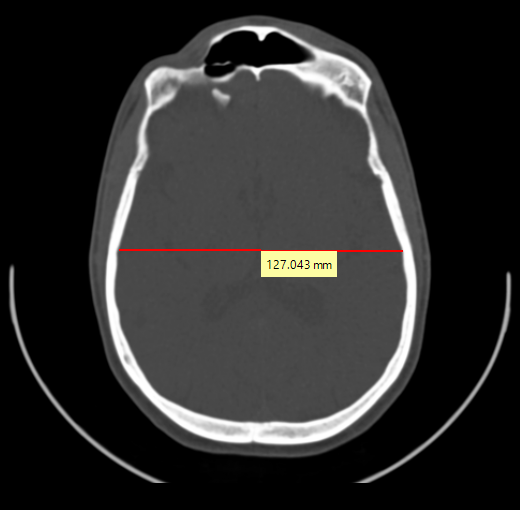
\includegraphics[scale=0.4]{axial_linear.png}
\caption{Linear measure on image}
\label{fig:axial_linear}
\end{figure}

\begin{figure}[!htb]
\centering
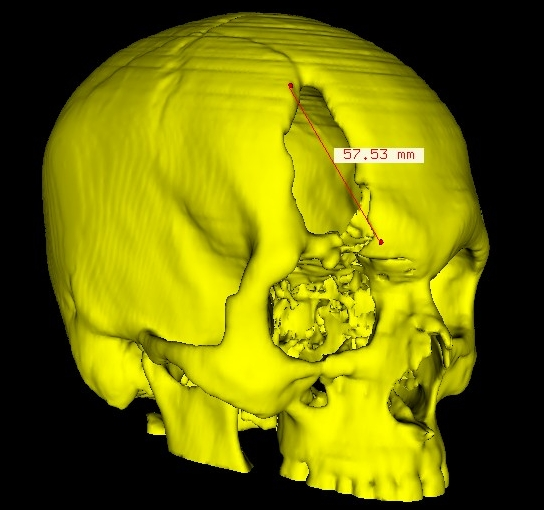
\includegraphics[scale=0.3]{3d_linear.jpg}
\caption{Linear measure on surface}
\label{fig:3d_linear}
\end{figure}

\textbf{Note: The linear measurement is given in millimeters (mm).}

\section{Angular Measurement}

An angular measurement in 2D on a surface (3D) can be done by clicking on the shortcut shown in figure~\ref{fig:atalho_angular}.

\begin{figure}[!htb]
\centering

\includegraphics[scale=0.2]{measure_angle_original}
\caption{Shortcut for angle measurement}
\label{fig:atalho_angular}
\end{figure}

To perform the angular measurement, is necessary to provide the three points that will describe the angle to be measured, A\^{B}C. Click \textbf{one} instead with the left button to determine the first point, A. To insert the second point, B (the vertex of the angle or the "center"), position the mouse pointer and click \textbf{one} again. Repeat the same actions to determine the third point, C. The resulting measurement is displayed on the image or surface.

The figure \ref{fig:axial_angular} illustrates an angular measurement on a flat image, and the figure \ref{fig:axial_superficie} illustrates an angular measurement on a surface.

As 2D linear measurement, you can also edit the 2D angular measurement, so you need to position the mouse on one end, hold down the \textbf{right mouse button} and drag it to the desired position.

\begin{figure}[!htb]
\centering
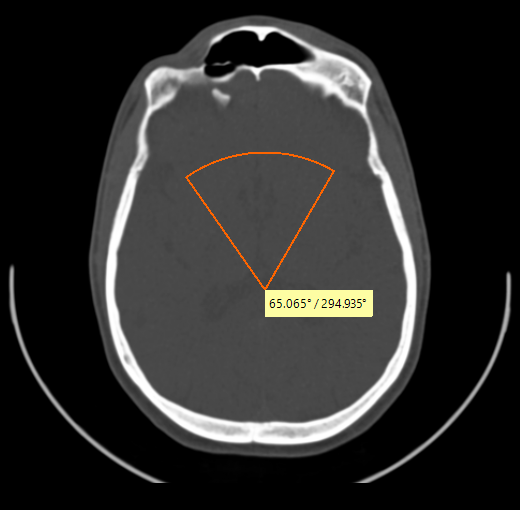
\includegraphics[scale=0.38]{axial_angular.png}
\caption{Angular measurement}
\label{fig:axial_angular}
\end{figure}

\begin{figure}[!htb]
\centering
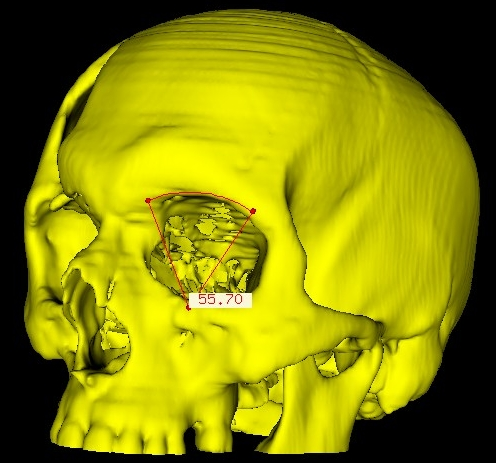
\includegraphics[scale=0.33]{angular_superficie.jpg}
\caption{Angular measurement on surface}
\label{fig:axial_superficie}
\end{figure}

\textbf{Note: Angular measurement is shown in degrees ($^{\circ}$)}


\section{Volumetric Measurement}

Volume and area measurements are made automatically when you create a new surface. they are displayed in the \textbf{Surfaces 3D} tab in the \textbf{Data} management panel, located in the corner
Bottom left of the screen, as illustrated in figure~\ref{fig:volumetric_mensure}.

\begin{figure}[!htb]
\centering
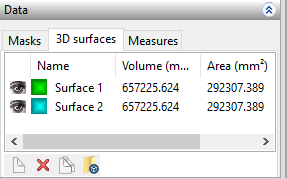
\includegraphics[scale=0.7]{painel_volumetric_measures_en.png}
\caption{Volumetric measurements}
\label{fig:volumetric_mensure}
\end{figure}

\textbf{Note: Volume measurement is given in cubic millimeter ($mm^3$), already the one of area in square millimeter ($mm^2$)}